\documentclass{standalone}
\usepackage{pgfplots}
\pgfplotsset{compat=1.18}
\usepgfplotslibrary{fillbetween}
\usepackage{amsmath}

\begin{document}

\definecolor{tab_blue}{HTML}{1F77B4}
\definecolor{tab_orange}{HTML}{FF7F0E}
\definecolor{tab_green}{HTML}{2CA02C}
\definecolor{tab_red}{HTML}{D62728}

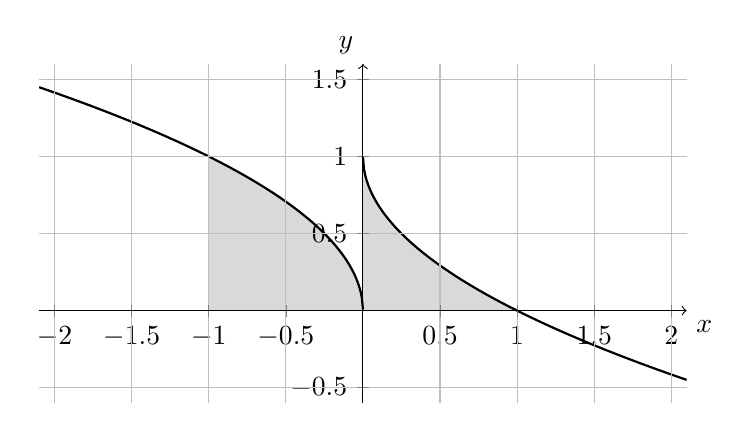
\begin{tikzpicture}[baseline]
\begin{axis}[
axis on top,
axis lines = middle,
unit vector ratio=1 1, 
% axis equal=false,
scale=1.2, 
xmin=-2.1, xmax=2.1, ymin=-0.6, ymax=1.6, 
grid = major,
% xtick={0, 1, 2, 3, 4},
% ytick={0, 1, 2, 3, 4},
xlabel=$x$,
ylabel=$y$,
xlabel style={below right},
ylabel style={above left},
axis line style = {->},
]

\addplot[samples=300, domain=-1:0, name path=func1] {sqrt(-x)};
\addplot[domain=-1:0, name path=axis1] {0}; 
\addplot[fill=gray!30] fill between [of=axis1 and func1]; 
\addplot[samples=300, domain=-2.1:0, thick] {sqrt(-x)};
\addplot[samples=300, domain=0:1, name path=func2] {1-sqrt(x)};
\addplot[domain=0:1, name path=axis2] {0}; 
\addplot[fill=gray!30] fill between [of=axis2 and func2]; 
\addplot[samples=300, domain=0:2.1, thick] {1-sqrt(x)};

% \addplot[samples=300, domain=-3:3, very thick] {1/(exp(x^2))};
% \legend{$y=e^{-x^2}$}
\end{axis}
\end{tikzpicture}

\end{document}